\begin{refsection}
    \renewcommand{\thefigure}{\arabic{figure}}
    \renewcommand{\thequadro}{\arabic{quadro}}
    
    \chapter[A utilização de modelos e analogias como estratégias de ensino e aprendizagem nas aulas de Química]{\marginpar{
        \begin{flushleft}
            \tiny \sffamily
            Artigo apresentado ao Curso de Pós-graduação do Instituto de Educação Superior Presidente Kennedy (IFESP) para obtenção do título de Especialista em Educação Matemática: teoria e prática no Ensino Fundamental. 
        \end{flushleft}
    }A utilização de modelos e analogias como estratégias de ensino e aprendizagem nas aulas de Química}
    \label{chap:utilizacao-modelos}
    
    \articleAuthor
    {Keila Barbosa da Fonseca}
    {Graduada em Química pela Universidade Federal do Rio Grande do Norte (UFRN). Mestra em Ensino de Ciências e Matemática (UFRN). E-mail: keilafonsec@hotmail.com}
    
    \articleAuthor
    {Lorena Gadelha de Freitas Brito}
    {Bacharela e Licenciada em Química (UFRN), licenciada em Pedagogia (UNINTER), metra em Ensino de Ciências e Matemática (UFRN) atualmente exerço a função de Professora Formadora do Instituto de Educação Superior Presidente Kennedy --- IFESP. ID Lattes: 0725.9511.9576.0694. E-mail: lorenagadelha@yahoo.com.br.}
    
    \begin{galoResumo}
        \marginpar{
            \begin{flushleft}
            \tiny \sffamily
            Como referenciar?\\\fullcite{SelfFonsecaAndBrito2021utilização}\mybibexclude{SelfFonsecaAndBrito2021utilização}, p. \pageref{chap:utilizacao-modelos}--\pageref{chap:utilizacao-modelosend}, \journalPubDate{}
            \end{flushleft}
        }
        Utilizar estratégias de ensino que promovam melhor compreensão de conceitos científicos, pelos alunos, é um desafio para muitos professores de Química da Educação Básica. O estudo do conteúdo, Geometria Molecular, necessário ao entendimento das interações intermoleculares, associado a outros conceitos, muitas vezes, é considerado pelos alunos de difícil compreensão. Nessa perspectiva, o uso de modelos e analogias como estratégias de ensino, podem contribuir com a aprendizagem, proporcionando momentos de reflexão, discussão e participação dos alunos sobre os fenômenos que compõem a natureza. Nesse sentido, a pesquisa tem como objetivo apresentar uma proposta didática sobre Geometria Molecular, utilizando, modelos e analogias com alunos do 1º ano do Ensino Médio da Escola Estadual Professor Edgar Barbosa, localizada na cidade de Natal-RN. Para a coleta de dados, foram utilizados princípios da pesquisa qualitativa e quantitativa e como instrumentos de pesquisa foi utilizado um questionário para avaliar os alunos, sobre o conteúdo proposto durante a unidade. Os resultados apontam que a proposta promoveu além da motivação, uma aprendizagem significativa no processo de ensino e da aprendizagem dos conteúdos abordados, que foi evidenciado através das atividades realizadas, como a criação de modelos concretos que possibilitou um maior envolvimento entre eles.
    \end{galoResumo}
    
    \galoPalavrasChave{Geometria molecular. Modelos. Analogias. Unidades didáticas.}
    
    \begin{otherlanguage}{english}

    \fakeChapterOneLine
    {Use of models and analogies as teaching-learning strategies in Chemistry classes}

    \begin{galoResumo}[Abstract]
        The use of education strategies that promote better understanding of scientific concepts to students can show itself to be quite challenging for many teachers of high schools. The study of the topic “Molecular Geometry”, needed to understand intermolecular relationships, associated with other concepts, is very often considered by the students to be difficult to comprehend. From this perspective, the use of models and analogies as teaching strategies can contribute to the learning, giving the students the opportunity to reflect and discuss natural phenomena. In this sense, the research has as an objective to present a didactic alternative to students taking the second year of high school at Escola Estadual Professor Edgar Barbosa, in Natal, Rio Grande do Norte, Brazil. Qualitative and quantitative research principles were used to collect data in a survey answered by the students. The replies show that the activities promoted significant improvement in students' learning, motivation and engagement.
    \end{galoResumo}
    
    \galoPalavrasChave[Keywords]{Molecular Geometry. Models. Analogies. Teaching Units.}
    \end{otherlanguage}

    \section{Introdução}

    No Ensino de Química, o grande número de conceitos abstratos, torna a disciplina bastante complexa e de difícil compreensão de uma série de fenômenos da natureza, despertando no professor a necessidade de utilizar novas ferramentas que possam contribuir para o entendimento dos alunos sobre diferentes conceitos. Nesse sentido, o uso de modelos e analogias, configura como um importante recurso/estratégia no processo de ensino e da aprendizagem dessa ciência e com essa abordagem, pode despertar um maior interesse dos alunos pela disciplina.  

    No meio educacional, discussões apontam para uma concepção diferenciada do conhecimento científico, sendo esse, relacionado com uma tentativa de compreensão e explicação de fenômenos do mundo natural. O desenvolvimento desse tipo de conhecimento utiliza constantemente representações que apresentam um caráter provisório, e são chamadas de modelos. De acordo com \textcite{GALAGOVSKYAndADÚRIZBRAVO2001Modelos}, os modelos são considerados ferramentas de representação teórica do mundo, auxiliando a sua explicação, predição e transformação. 

    Para este trabalho, foi abordado conceitos químicos relacionados a Geometria Molecular e polaridade das moléculas no 1º ano do Ensino Médio. Para desenvolver o estudo foi utilizado aulas expositivas e dialogadas, experimentais, modelos e analogias para explicar e fazer a mediação entre o conhecimento que o aluno já possui e os novos conceitos científicos que serão abordados neste artigo, buscando investigar, desse modo as possíveis potencialidades que essas ferramentas de ensino podem trazer para as aulas de Química.

    \section{Modelos e analogias no ensino de química e a aprendizagem significativa}

    O desenvolvimento de atividades baseadas na utilização de modelos, pode contribuir para a reflexão, discussão e participação dos alunos em sala de aula. A construção do conhecimento é favorecida, não somente pela apresentação dos modelos aos alunos, mas também pelo desenvolvimento de atividades que priorizem a construção de modelos representacionais, permitindo ao aluno utilizar os conhecimentos escolares em outras situações do seu cotidiano. Nessa perspectiva, a participação do professor durante esse processo é fundamental para criar possibilidades de produzi-lo e explorá-lo, contribuindo para uma melhor compreensão dos alunos de forma que esse recurso possa contribuir para a construção do conhecimento. 

    Consideradas importantes ferramentas no processo educativo, as analogias conferem poder discursivo ao conhecimento científico, dando uma nova visão do não observável, providenciando formas de argumentação. Nessa perspectiva, a Teoria da Aprendizagem Significativa (TAS) de David Ausubel, pode ajudar a reestruturar a memória já existente e prepará-la para novas informações.  

    De acordo com essa teoria, a nova informação interage em comum, à estrutura de conhecimento específico, chamada pelo autor de conceito \textit{subsunçor}. Quando o conteúdo escolar a ser aprendido não consegue ligar-se a algo já conhecido, ocorre uma aprendizagem mecânica, ou seja, as informações são aprendidas sem interagir com conceitos relevantes existentes na estrutura cognitiva. Assim, a pessoa decora fórmulas, leis, mas esquece após uma avaliação. Para haver aprendizagem significativa são necessárias duas condições. Em primeiro lugar, o aluno precisa ter uma disposição para aprender: se o indivíduo quiser memorizar o conteúdo arbitrária e literalmente, então a aprendizagem será mecânica. Em segundo, o conteúdo escolar a ser aprendido tem que ser potencialmente significativo \cite{AUSUBEL2000The}. 

    A utilização de recursos que facilitem a aquisição do conhecimento de forma significativa, por exemplo, uso de modelos e analogias, deve levar em conta a existência de subsunçores na estrutura cognitiva do aluno. Caso o novo conteúdo não encontre âncoras, podem ser utilizados conteúdos introdutórios com o objetivo de preencher a lacuna existente entre o que se sabe e o que se deseja que o aluno aprenda. Sobre a utilização de analogias, pode-se compreender que desempenham um papel importante na construção de um novo modelo que ultrapassa a dimensão do que é observável, contribuindo para a construção de um conhecimento novo \cite{MORTIMER2000Linguagem}.

    Para evitar o surgimento de concepções alternativas nos estudantes, o professor deve compreender que sua aplicação não é tão óbvia como muitos pensam, e para utilizá-las deve fazer uso do Modelo de Ensino com Analogias \textit{Teachinhg Wiht Analogies} (TWA), apresentado por \textcite{HARRISONAndTREAGUST1993Teaching}. 

    De acordo com Harrison e Treagust, a utilização desses modelos envolvem as seguintes etapas:

    \begin{quotation}
        Introdução do conceito alvo a ser aprendido, por meio de uma breve ou completa explicação de acordo com a analogia a ser empregada; Sugerir a situação análoga aos alunos e mediante discussões estimar a familiaridade dos estudantes com o análogo; Identificar as características relevantes do análogo; Mapear as similaridades entre alvo e análogo; Indicar onde a analogia falha, onde o análogo e o alvo não têm correspondência; Esboçar conclusões sobre o alvo \cite[p.~1291]{HARRISONAndTREAGUST1993Teaching}. 
    \end{quotation}

    Assim, a sequência dos passos propostos pelo Modelo TWA pode ser modificada segundo \textcite{HARRISONAndTREAGUST1993Teaching}, sofrendo influências de alguns fatores, tais como: estilo do professor; particularidades do conceito científico e o análogo que está sendo estudado, estimulando alunos a elaborar analogias, tendo em vista que o desenvolvimento dessa atividade pode contribuir para explicar e compreender não somente o conteúdo Geometria Molecular, mas diversos conteúdos presentes no Ensino da Química. 

    \section{Vantagens e desvantagens do trabalho com modelos e analogias}

    A palavra modelo pode apresentar diferentes significados, tais como: tipo de objeto, padrão a seguir, exemplo de perfeição, representação concreta de um objeto capaz de reproduzir suas principais características visuais e estruturais, dentre outros. Em um contexto científico, \textcite{GILBERT2004Models} considera que um modelo é a representação parcial de um objeto, um evento, um processo ou uma ideia, criado com objetivo específico. Nesse sentido, os modelos, criações da mente humana, são representações que apresentam contribuições no ensino de ciências desempenhando vários objetivos, tais como: simplificar entidades complexas, contribuir com a comunicação de ideias, favorecer a visualização de entidades abstratas e fundamentar a proposição e a interpretação de experimentos sobre a realidade. 

    \textcite{DUARTE2005Analogias} em seu trabalho apresenta algumas potencialidades sobre o uso de analogias que ativam o raciocínio analógico, organizam a percepção, desenvolvem capacidades cognitivas como a criatividade e a tomada de decisão, que tornam o conhecimento científico mais inteligível e plausível, facilitando a compreensão, a visualização de conceitos abstratos, podendo promover o interesse dos alunos e podem ser utilizadas para avaliar o conhecimento e a compreensão dos alunos.  

    Algumas dificuldades podem ocorrer a partir dessas analogias, como: a analogia pode ser interpretada como o conceito em estudo, ou dela serem apenas retidos os detalhes mais evidentes e apelativos, sem se chegar a atingir o que se pretendia; podem não ocorrer um raciocínio analógico que leve a compreensão da analogia; a analogia pode não ser reconhecida como tal, não ficando explícita a sua utilidade; os alunos podem centrar-se nos aspectos positivos da analogia e desvalorizar as suas limitações. Dessa forma, compreende-se que a compreensão dos conceitos científicos na Química e em outras ciências que depende do domínio de uma série de habilidades como raciocínio abstrato, domínio da linguagem simbólica, podem ser favorecidos pelo uso dessa estratégia de ensino. 

    \section{Elaboração de uma sequência didática}

    Uma unidade didática ou sequência didática é um trabalho que compreende a escolha de estratégias de ensino que contribuam para a construção de um conhecimento mais significativo \cite{CAAMAÑO2011Enseñar}.

    Segundo \textcite{ZABALA1998prática} sequência didática é um encadeamento de passos ou etapas ligadas entre si, para tornar mais eficiente o processo de aprendizagens planejadas e desenvolvidas com objetivos educacionais específicos com início, meio e fim conhecido tanto por professores quanto por alunos. Nessa perspectiva, é fundamental o envolvimento de todos, cabendo ao professor o papel de mediador durante a ação de construção do conhecimento e necessitando dos alunos a disponibilidade e o interesse de aprender. A estruturação da aula a partir de uma Unidade didática favorece a criatividade, a flexibilidade e inovação, fatores que podem contribuir com o desenvolvimento da autonomia do aluno. Nesse sentido pode-se dizer que o aluno tem a oportunidade de \textit{aprender a aprender}.  

    O desenvolvimento de uma unidade didática é um processo complexo, que pode tomar vários caminhos e envolve em seu planejamento, tomada de decisão que implica na escolha dos objetivos, seleção e organização dos conteúdos, sequências de atividades, seleção de atividades de avaliação, organização e gestão da aula.  

    \section{Procedimentos metodológicos}

    A pesquisa se enquadra em uma perspectiva qualitativa e quantitativa, baseada na pesquisa-ação que envolve a análise de dados escritos, ações e comunicações dos participantes reunidos através da utilização de instrumentos de coletas de dados. De acordo com \textcite{FLICK2009Introdução} a pesquisa qualitativa considera as observações realizadas no cotidiano e no contexto social como importantes para investigação. Caracterizada como uma pesquisa-ação em que o pesquisador e participantes estão envolvidos de modo cooperativo e participativo.  

    O público-alvo da pesquisa foram trinta e nove alunos do Ensino Médio da Escola Estadual Professor Edgar Barbosa localizada no Município do Natal/RN. Para investigar as concepções dos alunos sobre os modelos, foi aplicado, um questionário e os resultados obtidos foram organizados em gráficos e quadros. 

    \section{Resultados e discussões}

    A sequência didática elaborada foi aplicada em 3 encontros, totalizando 6 aulas de cinquenta minutos cada. Foram abordados os conteúdos envolvendo Geometria Molecular e interações intermoleculares. As atividades realizadas e os recursos utilizados em cada encontro serão descritos a seguir. 

    Com o objetivo de levantar as concepções prévias acerca do termo \textit{modelo} e sua utilização nas aulas de Química, inicialmente foi aplicado com 39 alunos identificados como A1 a A39 um questionário sobre o tema, envolvendo os diferentes significados que o termo \textit{modelo} pode assumir na Língua Portuguesa. Algumas ideias expressadas pelos alunos, merecem destaque e serão apresentadas a seguir: \textit{Modelo seria uma representação de algo como modelo de revistas que representa marcas de roupas ou modelo de Thomson que representa sua forma de ver o átomo} (A27). \textit{Tipo um exemplo, algo a ser seguido, que serve para visualizar e aprender. É importante sim, aprendo mais com ele} (A32). \textit{Modelo é um exemplo aproximado de algo. Ex: Modelo das fitas de DNA} (A11).  

    Após o levantamento das ideias prévias dos alunos participantes da pesquisa, imagens relacionadas aos diferentes significados da palavra foram apresentadas por meio de slides que representavam os diferentes significados que o termo modelo pode assumir e suas características. 

    Em seguida foi trabalhado com os alunos o conteúdo de Ligações Químicas, que de acordo com \textcite{FERNANDEZAndMARCONDES2006Concepções} os conceitos abordados sobre Ligações Químicas, estão bem relacionados com a constituição da matéria, ou seja, conceitos abstratos e, consequentemente, demandam dos alunos um desenvolvimento cognitivo mais próximo do lógico-formal, um pensamento abstrato mais organizado. Dessa forma, com o propósito de favorecer uma compreensão mais adequada do assunto foram utilizadas estratégias como apresentação de um vídeo sobre: condutividade elétrica dos materiais, e atividades de modelagem.  

    Inicialmente, os alunos assistiram o vídeo e em seguida, após a apresentação foi realizado a seguinte questionamento: Por que o cloreto de sódio conduziu corrente elétrica quando em solução aquosa e não conduziu corrente no estado sólido? As concepções iniciais dos alunos podem ser vistas a seguir: \textit{É que a água é um condutor, mas mostra que a água não conduz} (A32). \textit{Modificou a estrutura do sólido, nesse caso está mais comprimido como se estivesse de uma forma e quando colocou na água formou um novo tipo que conduziu} (A3). \textit{Eu acho que mudou o estado físico, como se tivesse aberto espaço} (A22).

    De acordo com \textcite{MACHADOAndMORTIMER2007Química} o conhecimento químico é construído pela combinação de três níveis representacionais: fenomenológico, teórico e representacional, o que pode ser traduzido para realização de uma discussão nas dimensões: macroscópica, submicroscópica e simbólica. De acordo com \textcite{MORAIS2007Recurso} a utilização de modelos para intermediar o aprendizado, é simples e ajuda os alunos a desenvolver a percepção do arranjo espacial das ligações químicas existentes entre os núcleos atômicos que compõem uma molécula. O quadro 1 mostra os resultados das estruturas criadas pelos alunos com diferentes materiais para representar diferentes moléculas.

    \begin{longquadro}[t]{ | c m{.26\textwidth} c c |}
    
        \caption{Estruturas criadas pelos alunos e materiais utilizados na atividade proposta}
        \label{quad:estruturas-quimicas}\\
       
        \hline
        Estruturas criadas & Materiais utilizados & Geometria & Nomenclatura\\
        \hline
        \endfirsthead

        \multicolumn{4}{c}{\footnotesize \textsf{Quadro \ref{quad:estruturas-quimicas}~--~\textit{Estruturas criadas pelos alunos e materiais utilizados na at\dots (continuação)}}\medskip }\\
        \hline
        Estruturas criadas & Materiais utilizados & Geometria & Nomenclatura\\
        \hline
        \endhead

        \multicolumn{4}{r}{\footnotesize \textsf{\textit{continua}}}\\
        \endfoot
       
        \hline
        \caption*{Fonte: elaboração da autora}
        \endlastfoot

        \makecell{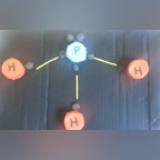
\includegraphics[width=0.20\textwidth]{articles/06-utilizacao-de-modelo/quadro1-1.jpeg}}%
            & \begin{itemize}[series=nospace,nosep,leftmargin=*,after=\vspace{-\baselineskip},before=\vspace{-\baselineskip}]%
                \item Tampas de garrafa%
                \item Palitos de madeira%
                \item Lã de aço%
                \item Papelão%
                \item Tinta%
            \end{itemize} %%
            & \makecell{Piramidal} %
            & \makecell{\ce{PH3}\\(Hidreto de fósforo)} \\

        \hline

        \makecell{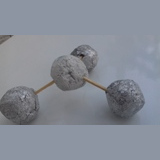
\includegraphics[width=0.20\textwidth]{articles/06-utilizacao-de-modelo/quadro1-2.jpeg}}%
            & \begin{itemize}[series=nospace,nosep,leftmargin=*,after=\vspace{-\baselineskip},before=\vspace{-\baselineskip}]%
                \item Folha de alumínio%
                \item Palitos de madeira%
            \end{itemize} %%
            & \makecell{Piramidal} %
            & \makecell{\ce{NH3}\\(Amônia)}\\

        \hline

        \makecell{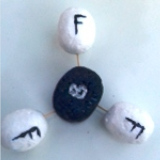
\includegraphics[width=0.20\textwidth]{articles/06-utilizacao-de-modelo/quadro1-3.jpeg}}%
            & \begin{itemize}[series=nospace,nosep,leftmargin=*,after=\vspace{-\baselineskip},before=\vspace{-\baselineskip}]
                \item Bolinhas de isopor
                \item Palitos de madeira
                \item Tinta
            \end{itemize} %%
            & \makecell{Trigonal\\plana} %
            & \makecell{\ce{BF3}\\(Trifluoreto de boro)} \\

        \hline

        \makecell{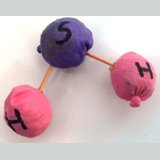
\includegraphics[width=0.20\textwidth]{articles/06-utilizacao-de-modelo/quadro1-4.jpeg}}%
            & \begin{itemize}[series=nospace,nosep,leftmargin=*,after=\vspace{-\baselineskip},before=\vspace{-\baselineskip}]
                \item Bexiga de ar
                \item Arroz
                \item Caneta colorida
                \item Palito de madeira
            \end{itemize} %%
            & \makecell{Angular} %
            & \makecell{\ce{H2S}\\(Ácido sulfídrico)} \\

        \hline

        \makecell{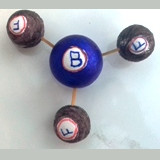
\includegraphics[width=0.20\textwidth]{articles/06-utilizacao-de-modelo/quadro1-5.jpeg}}%
            & \begin{itemize}[series=nospace,nosep,leftmargin=*,after=\vspace{-\baselineskip},before=\vspace{-\baselineskip}]
                \item Bolinhas de isopor
                \item Palitos de madeira
                \item Tinta
            \end{itemize} %%
            & \makecell{Trigonal\\plana} %
            & \makecell{\ce{BF3}\\(Trifluoreto de boro)} \\

        \hline

        \makecell{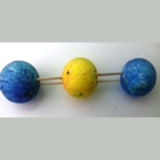
\includegraphics[width=0.20\textwidth]{articles/06-utilizacao-de-modelo/quadro1-6.jpeg}}%
            & \begin{itemize}[series=nospace,nosep,leftmargin=*,after=\vspace{-\baselineskip},before=\vspace{-\baselineskip}]
                \item Bolinhas de isopor
                \item Palitos de madeira
                \item Tinta
            \end{itemize} %%
            & \makecell{Linear} %
            & \makecell{\ce{CO2}\\(Gás carbônico)} \\

        \hline

        \makecell{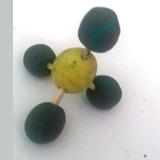
\includegraphics[width=0.20\textwidth]{articles/06-utilizacao-de-modelo/quadro1-7.jpeg}}%
            & \begin{itemize}[series=nospace,nosep,leftmargin=*,after=\vspace{-\baselineskip},before=\vspace{-\baselineskip}]%
                \item Massa de modelar%
                \item Palitos de madeira%
            \end{itemize} %%
            & \makecell{Tetraédrica} %
            & \makecell{\ce{CH4}\\(Gás metano)} \\

        \hline

        \makecell{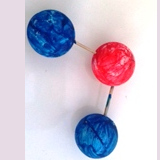
\includegraphics[width=0.20\textwidth]{articles/06-utilizacao-de-modelo/quadro1-8.jpeg}}%
            & \begin{itemize}[series=nospace,nosep,leftmargin=*,after=\vspace{-\baselineskip},before=\vspace{-\baselineskip}]
                \item Bolinhas de isopor
                \item Palitos de madeira
                \item Tinta
            \end{itemize} %%
            & \makecell{Angular} %
            & \makecell{\ce{H2O}\\(Água)} \\

        \hline

        \makecell{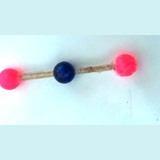
\includegraphics[width=0.20\textwidth]{articles/06-utilizacao-de-modelo/quadro1-9.jpeg}}%
            & \begin{itemize}[series=nospace,nosep,leftmargin=*,after=\vspace{-\baselineskip},before=\vspace{-\baselineskip}]
                \item Miçangas
                \item Palitos de madeira
                \item Fita adesiva
            \end{itemize} %%
            & \makecell{Linear} %
            & \makecell{\ce{CO2}\\(Gás carbônico)} \\
    \end{longquadro}

    Através dos modelos elaborados, foi observado que os grupos utilizaram os mais diversos materiais em suas produções e a maioria deles expressou de forma coerente as ligações existentes entre os átomos. Apenas dois grupos apresentaram dificuldades em representar de forma correta o arranjo espacial. Nesse sentido, a confecção dos modelos contribuiu para o processo de formação conceitual sobre a disposição dos átomos na representação de uma molécula, tendo em vista que a partir de uma estratégia como essa foi possível perceber que os alunos visualizassem as estruturas de forma tridimensional. Após a apresentação dos modelos, os alunos preencheram uma tabela no caderno representando os modelos construídos e suas respectivas geometrias.  

    No encontro seguinte foi abordado o conceito de solubilidade, já que a partir dele é possível compreender outros conceitos químicos, como as interações existentes entre as moléculas das substâncias. Nesse sentido, foi realizado um experimento envolvendo diferentes substâncias e a partir dos resultados obtidos com a atividade experimental os alunos, responderam as seguintes questões: 

    \begin{enumerate}
        \item Os materiais moleculares apresentam o mesmo comportamento com relação à dissolução? 
        \item Quais as substâncias ou produtos comerciais (água, óleo de soja, vaselina ou parafina e vinagre) têm comportamento semelhante ao do sal de cozinha? 
        \item Ocorre ou não dissolução entre materiais moleculares? Que conclusões você pode extrair desse experimento?
    \end{enumerate}

    Os resultados obtidos com os questionamentos podem ser observados nos gráficos das Figuras \ref{fig:resp-q1-quim}, \ref{fig:resp-q2-quim} e \ref{fig:resp-q3-quim}.
    
    \begin{figure}[ht]%
        \centering%
        \caption{Respostas dos alunos à Questão 1}%
        \begin{tikzpicture}
            \pie[text=legend, radius=2]{74/Comportamento distinto,
                12/Comportamento semelhante,
                14/Não responderam}
        \end{tikzpicture}
        \caption*{Fonte: Elaborado pela autora.}%
        \label{fig:resp-q1-quim}%
    \end{figure}%

    \begin{figure}[ht]%
        \centering%
        \caption{Respostas dos alunos à Questão 2}%
        \begin{tikzpicture}
            \pie[text=legend, radius=2]{54/Água e vinagre,
                26/Somente o vinagre,
                3/Todas,
                17/Não responderam}
        \end{tikzpicture}
        \caption*{Fonte: Elaborado pela autora.}%
        \label{fig:resp-q2-quim}%
    \end{figure}%

    \begin{figure}[ht]%
        \centering%
        \caption{Respostas dos alunos à Questão 3}%
        \begin{tikzpicture}
            \pie[text=legend, radius=2]{49/Depende da polaridade,
                23/Ocorre,
                17/Não ocorre,
                11/Não responderam}
        \end{tikzpicture}
        \caption*{Fonte: Elaborado pela autora.}%
        \label{fig:resp-q3-quim}%
    \end{figure}%

    Na sequência construíram modelos concretos utilizando materiais alternativos para representar as interações existentes entre as substâncias, o resultado do trabalho realizado por eles, pode ser visto no Quadro \ref{quad:modelos-quimicos}.

    Na elaboração dos modelos, os alunos utilizaram os mais diversos materiais, desde papel cortado em tiras até flocos de arroz tingidos. De acordo com \textcite{JUSTI2006enseñanza} a aprendizagem por meio de modelos pode ter lugar em dois momentos do processo: na construção (modelagem) e na utilização do modelo, visto que quando um modelo é construído, cria-se um tipo de estrutura representativa, desenvolvendo, assim, uma forma científica de pensar, bem como também, aprende-se sobre a situação representada.

    \begin{longquadro}[t]{ | c m{.30\textwidth} c |}
    
        \caption{Modelos criadas pelos alunos}
        \label{quad:modelos-quimicos}\\
       
        \hline
        Modelos criadas & Material utilizado & Sistemas representados\\
        \hline
        \endfirsthead

        \multicolumn{3}{c}{\footnotesize \textsf{Quadro \ref{quad:modelos-quimicos}~--~\textit{Modelos criadas pelos alunos (continuação)}}\medskip }\\
        \hline
        Modelos criadas & Material utilizado & Sistemas representados\\
        \hline
        \endhead

        \multicolumn{3}{r}{\footnotesize \textsf{\textit{continua}}}\\
        \endfoot
       
        \hline
        \caption*{Fonte: elaboração da autora}
        \endlastfoot

        \makecell{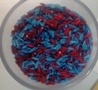
\includegraphics[width=0.20\textwidth]{articles/06-utilizacao-de-modelo/quadro2-1.jpeg}}%
            & Arroz tingido nas cores azul e vermelho%
            & \makecell{Mistura homogênea}\\
        \hline

        \makecell{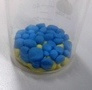
\includegraphics[width=0.20\textwidth]{articles/06-utilizacao-de-modelo/quadro2-2.jpeg}}%
            & Massa de modelar nas cores azul e amarelo%
            & \makecell{Mistura heterogênea}\\
        \hline

        \makecell{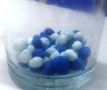
\includegraphics[width=0.20\textwidth]{articles/06-utilizacao-de-modelo/quadro2-3.jpeg}}%
            & Massa de modelar nas cores azul e branco%
            & \makecell{Mistura homogênea}\\
        \hline

        \makecell{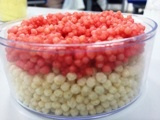
\includegraphics[width=0.20\textwidth]{articles/06-utilizacao-de-modelo/quadro2-4.jpeg}}%
            & Flocos de arroz nas cores vermelho e amarelo%
            & \makecell{Mistura heterogênea}\\

        \hline

        \makecell{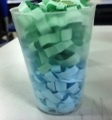
\includegraphics[width=0.20\textwidth]{articles/06-utilizacao-de-modelo/quadro2-5.jpeg}}%
            & Tiras de papel nas cores azul e verde%
            & \makecell{Mistura heterogênea}\\

        \hline

        \makecell{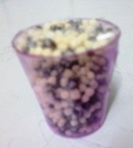
\includegraphics[width=0.20\textwidth]{articles/06-utilizacao-de-modelo/quadro2-6.jpeg}}%
            & Cereais de chocolate ao leite e chocolate branco%
            & \makecell{Mistura homogênea}\\

        \hline

        \makecell{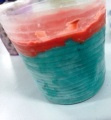
\includegraphics[width=0.20\textwidth]{articles/06-utilizacao-de-modelo/quadro2-7.jpeg}}%
            & Massa de modelar nas cores laranja e verde%
            & \makecell{Mistura heterogênea}\\

        \hline

        \makecell{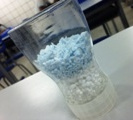
\includegraphics[width=0.20\textwidth]{articles/06-utilizacao-de-modelo/quadro2-8.jpeg}}%
            & Flocos de isopor nas cores azul e branco%
            & \makecell{Mistura heterogênea}\\

    \end{longquadro}

    \section{Considerações finais}

    Através das estratégias e recursos utilizados na elaboração das atividades, foi observado que a maioria dos alunos envolvidos conseguiram desenvolver uma boa compreensão dos conceitos abordados nessa proposta de ensino  

    A sequência didática para o Ensino de Química foi bem aceita pelos alunos, possibilitando a interação e a socialização das ideias, motivando-os e despertando o interesse dos diversos conteúdos abordados nas aulas, elementos que foram importantes para a construção do conhecimento em sala de aula.  

    Portanto, diante do que foi exposto, se faz necessário uma reflexão pelos professores de Química sobre a utilização de estratégias de ensino, como o uso de modelos e analogias durante as aulas, e as contribuições que a utilização dessas estratégias pode trazer ao processo de ensino e aprendizagem da Química no Ensino Médio.  

    \nocite{NOVAK1991Ayudar}
    \nocite{NUNESAndFERRAZDAndJUSTINA2007Estudos}

    \printbibliography[heading=subbibliography,notcategory=fullcited]

    \label{chap:utilizacao-modelosend}

\end{refsection}
